\documentclass[11pt,a4paper]{article}

\usepackage[margin=1.8cm]{geometry}
\usepackage[T1]{fontenc}
\usepackage{lmodern}
\usepackage{microtype}
\usepackage{booktabs}
\usepackage{tabularx}
\usepackage{enumitem}
\usepackage{xcolor}
\usepackage{float}
\usepackage{pgfplots}
\usepackage[hidelinks]{hyperref}
\pgfplotsset{compat=1.16}

\setlist{nosep,leftmargin=*}
\setlength{\parskip}{3pt}
\setlength{\parindent}{0pt}
\newcommand{\code}[1]{\texttt{\small #1}}

\title{\vspace{-1.6cm}\textbf{ReportLens: Uncertainty-Aware Verification of\\Number-Based Chart Claims in Student Technical Reports}\\[4pt]
\large Mid-Submission Report \,--\, LMA Group Project 2026}
\author{\begin{tabular}{ll}
Harsh Raj (2025202005) & \hspace{2em}Hritik Ranjan (2025202031) \\
Karan Thayat (2025202008) & \hspace{2em}Vikash Kumar (2025201012)
\end{tabular}}
\date{\vspace{-10pt}31 October 2026\vspace{-8pt}}

\begin{document}
\maketitle

\begin{center}
\textbf{GitHub repository:} \url{https://github.com/IIITH-2025-27/ReportLens}
\end{center}

\section{Overview}

ReportLens (Python package \code{chart\_claim\_verifier}) checks whether the numbers a student writes in a report match the report's own charts. A sentence such as ``accuracy reaches 0.82 at epoch 10 (Figure 3)'' is matched to its figure, parsed into a checkable claim, and the chart value is read by four independent tools. The spread of those readings is calibrated on charts with known values, so a claim is flagged only when the gap is clearly larger than the reading error. Unclear cases go to the TA instead of becoming a wrong accusation.

The pipeline has five stages: (1) \textbf{find the figure} (BM25 + coverage check, or ``no matching figure''); (2) \textbf{parse the claim} into series, x-point, value and allowed rounding (rules first, LLM only when rules fail); (3) \textbf{measure} with a VLM crop reader, a VLM chart-to-table pass, DePlot, and OCR + pixel measurement, taking the median; (4) \textbf{calibrate} tool disagreement into an error margin with conformal calibration; (5) \textbf{decide} with a fixed, tested rule (Consistent / Mismatch / Not sure / No matching figure), with Benjamini--Hochberg controlling the wrong-flag rate over a batch. The language model parses sentences and chooses the next tool, but it never decides a verdict.

\textbf{Headline result so far.} On 1{,}000 claims from 100 reports, the informed agent decides 78.6\% of claims, is right on 96.8\% of those it decides, and wrongly flags 3.0\% [1.4, 4.8] of correct claims, well under the 10\% target set in the proposal. It does this with 35--40\% of the model time of running every tool.

\section{Progress so far}

All modules in the plan are built and merged (git history 15--29 October 2026) and covered by 67 unit and end-to-end tests (Table~\ref{tab:status}). Every experiment runs locally with Qwen3-VL-4B, on Apple-silicon MPS or a CUDA T4.

\textbf{Change from the proposal.} The image-retrieval model is not used in the current runs (an embedding scorer can still be plugged in): a cited figure number plus caption and legend text, with a VLM legend reader for near-misses, already brings retrieval errors on dev from 9 to 2 and on test from 4 to 0.

\begin{table}[H]
\centering\footnotesize
\caption{Implementation status of each component.}
\label{tab:status}
\begin{tabular}{lll}
\toprule
Component & Module & State \\
\midrule
Synthetic generator (charts, PDF reports, claims, injections) & \code{generator/} & done \\
PDF ingest; figure retrieval (BM25, cited figure, legend names) & \code{ingest/}, \code{retrieval/} & done \\
Claim finder, rule parser, LLM fallback parser, rounding rules & \code{claims/} & done \\
Tools: VLM crop, VLM chart-to-table, DePlot, OCR + pixel reader & \code{tools/} & done \\
Conformal calibration, decision rule, Benjamini--Hochberg check & \code{calibration/}, \code{decide/} & done \\
Agent: tool profile, informed planner, memory, repair; policies P0--P3 & \code{agent/} & done \\
VLM baselines B1--B4; coverage sweep B5 & \code{baselines/} & runs pending \\
Mock LMS with action guard; safety metrics & \code{lms/}, \code{evaluation/} & done \\
LoRA chart-to-table adapter for the VLM table tool & \code{finetune/} & trained, evaluated \\
\bottomrule
\end{tabular}
\end{table}

\section{Datasets}

All evaluation data is synthetic and produced by our generator, so the true value behind every sentence is known. Tables that look like student ML results are plotted as line, bar and grouped-bar charts in varied styles and placed into short PDF reports. Claims come from the same tables: true claims (some rounded), claims with a planted error of 2--50\% of the value, mix-ups such as a wrong series, and claims no figure shows. About 15\% of reports carry hidden instructions for the safety test. Splits are made by report and by source table, so nothing appears in two splits.

\begin{center}\small
\begin{tabularx}{\linewidth}{lrlX}
\toprule
Split & Reports & Size & Purpose \\
\midrule
calib + calib\_easy & 12 + 5 & 51 figures, 1{,}063 points & Fit error margins and the tool profile \\
dev & 20 & 208 claims & Development (design choices made here) \\
test & 20 & 201 claims & Development (design choices made here) \\
holdout & 20 & 186 claims & Frozen-config run, later used to diagnose calibration \\
holdout2 & 20 & 208 claims & Fresh; only two bug fixes after viewing it \\
holdout3 & 20 & 197 claims & Fresh; used once to pick between two calibration tables \\
phrasing & 10 & -- & Unusual wordings, for the parse stage only \\
ft\_pool & 370 & $\approx$1{,}100 charts & LoRA fine-tuning data, no injected text \\
\bottomrule
\end{tabularx}
\end{center}

The evaluated pool (100 reports, 1{,}000 claims) matches the proposal's planned 1{,}000-sentence test. Calibration (17 reports vs.\ 60 planned) and the fine-tuning pool ($\approx$1{,}100 vs.\ 6{,}000 charts) are smaller because all runs are on local hardware. Real claims from SciVer and MuSciClaims are not yet used.

\section{Baseline experiments}

\textbf{Tool-policy baselines (run).} All use the same tools, calibration and decision rule; only the choice of which tools to call differs:
\begin{itemize}
\item \textbf{P0 \code{all\_tools}}: read every value with all four tools.
\item \textbf{P1 \code{fixed\_order}}: call tools in a fixed order (OCR+pixel, DePlot, VLM table, VLM crop) until the rule can decide.
\item \textbf{P3 \code{informed} (main method)}: plan a trustworthy \emph{pair} of tools per figure from the measured profile, read the member most likely to fail first, remember failures, and repair when a repair was measured to work.
\end{itemize}

\textbf{Tool profile (calibration charts, pooled).} Each tool's reading quality, measured on calibration charts with known values. Errors are a fraction of the axis range; a ``big error'' is above 5\%.

\begin{center}\small
\begin{tabular}{lrrrr}
\toprule
Tool & Success & Median error & Big errors & Time per figure \\
\midrule
OCR + pixel & 50.3\% & 0.15\% & 0.9\% & 0.04 s \\
DePlot & 66.8\% & 0.24\% & 4.6\% & 8.9 s \\
VLM chart-to-table & 66.2\% & 1.40\% & 26.0\% & 16.6 s \\
VLM crop & 100\% & 1.63\% & 25.1\% & 52.8 s \\
\bottomrule
\end{tabular}
\end{center}

The pixel reader is the most accurate but refuses often (42\% success on hard line charts); the VLM crop always answers but is badly wrong a quarter of the time. What matters for the rule is how often two tools agree on a \emph{wrong} value: OCR+pixel with DePlot agree wrongly 0.2\% of the time, while the two VLM tools (same model) agree wrongly 2.7\% of the time (5.1\% on hard line charts). The informed planner therefore never uses the two VLM tools as each other's cross-check.

\textbf{VLM baselines (implemented, runs pending).} B1 direct verdict, B2 direct verdict with stated confidence, B3 majority vote over samples, B4 the model using our tools freely and giving its own verdict, and B5 the coverage-at-10\%-wrong-flags sweep. These are implemented in \code{baselines/vlm\_baselines.py} and \code{evaluation/sweep.py} and are the first item of the remaining timeline.

\section{Ablations}

Each change was measured on saved readings or a live run before it was kept; the full log is in \code{results/run\_log.md}.

\begin{center}\small
\begin{tabularx}{\linewidth}{lXXc}
\toprule
ID & Change & Measured effect & Kept \\
\midrule
U11a & Use a cited ``Figure N'' when OCR misses the series name & 6 of 13 wrong NO\_FIGURE fixed; 0 of 23 right ones changed & yes \\
U11b & Ask the VLM for legend names of near-miss figures & retrieval errors dev 9$\to$2, test 4$\to$0; P3 accuracy when decided dev 92.9$\to$97.0\% & yes \\
U10 & No reading when both legs of a difference read the same & dev wrong flags P3 2.9$\to$1.4\%; coverage $-0.5$ pt & yes \\
U16 & LLM parser accepts an epoch written as a number & parse failures 24$\to$0; field accuracy 66$\to$87--89\%; LLM calls 75$\to$51 & yes \\
-- & Hand off a claim when two figures fit & $-3$ pt coverage on test, one missed error removed & yes \\
B4 & Join sentences cut by a page break; reject cut comparisons & holdout2 wrong flags 3.6$\to$1.2\% & yes \\
U14 & Margins fitted per tool set & dev wrong flags 1.4$\to$4.1\% & no \\
-- & One vote per model (average the two VLM tools) & test coverage 70.2$\to$67.2\%; removes 2 wrong flags but 9 right ones & no \\
U17 & 34 more grouped-bar calibration charts & wrong flags test 1.2$\to$2.4\%, holdout3 3.0$\to$5.7\% & no \\
U18 & Legend-occlusion guard & saves 2 wrong flags, loses $\approx$50 true catches & no \\
E5 & Tool policy: P0 vs.\ P1 vs.\ P3 & see Table~\ref{tab:main} & -- \\
E6 & LoRA chart-to-table adapter for the VLM table tool & see Section~\ref{sec:lora} & open \\
\bottomrule
\end{tabularx}
\end{center}

\section{Results}

\begin{table}[H]
\centering\small
\caption{All five splits pooled (1{,}000 claims). 95\% bootstrap intervals resample whole reports. Wrong flags = share of correct claims flagged as wrong.}
\label{tab:main}
\begin{tabular}{lcccc}
\toprule
Policy & Coverage & Accuracy when decided & Wrong flags & Missed errors \\
\midrule
P0 all\_tools & 75.5\% [72.0, 78.9] & 95.6\% [93.9, 97.2] & 4.4\% [2.2, 6.9] & 1.3\% [0.4, 2.4] \\
P1 fixed\_order & 79.5\% [75.8, 83.2] & 96.4\% [94.8, 97.7] & 3.2\% [1.4, 5.2] & 1.3\% [0.4, 2.5] \\
\textbf{P3 informed} & 78.6\% [74.8, 82.5] & \textbf{96.8\%} [95.4, 98.0] & \textbf{3.0\%} [1.4, 4.8] & \textbf{0.6\%} [0.0, 1.5] \\
\bottomrule
\end{tabular}
\end{table}

The informed policy has the lowest wrong-flag and missed-error rates, with coverage within a point of P1, and it uses the least model time on every split (e.g.\ 16.6 min vs.\ 44.0 min for P0 on test). Its advantage over P1 is within the intervals, so it is not yet a significant win on accuracy; the clear win is cost.

\textbf{Per split (P3).} Coverage / accuracy when decided / wrong flags: test 74.1 / 99.3 / 1.2\%; dev 80.8 / 97.6 / 1.4\%; holdout 78.0 / 91.7 / 9.4\%; holdout2 83.7 / 97.7 / 1.2\%; holdout3 76.1 / 97.3 / 3.0\%. The two fresh splits (holdout2, holdout3) agree with the development splits; \code{holdout} is the outlier (Section~\ref{sec:challenges}). By chart type, bar and grouped-bar claims are decided 90--98\% of the time, while about 40\% of line-chart claims are handed to the TA.

\textbf{How small an error is caught.} Figure~\ref{fig:catch} shows the share of planted errors flagged by P3, pooled over the five splits. Half or more of the errors are caught at every size, down to 2\% of the value (45 of 74). Of the errors that received at least two readings, 79\% of the 2\% errors and 98\% of the 50\% errors are flagged; the rest are mostly handed off, not accepted.

\begin{figure}[H]
\centering
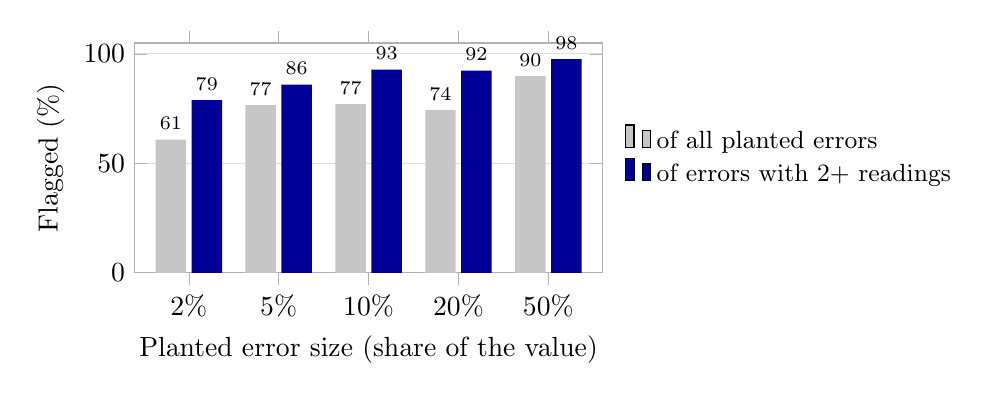
\begin{tikzpicture}
\begin{axis}[
  width=0.62\linewidth, height=4.5cm,
  ybar, bar width=11pt,
  ymin=0, ymax=105,
  ylabel={Flagged (\%)}, xlabel={Planted error size (share of the value)},
  symbolic x coords={2\%,5\%,10\%,20\%,50\%}, xtick=data,
  legend style={at={(1.03,0.5)},anchor=west,font=\small,draw=none},legend cell align=left,
  nodes near coords, nodes near coords style={font=\scriptsize},
  every node near coord/.append style={/pgf/number format/fixed,/pgf/number format/precision=0},
  ymajorgrids, grid style={gray!25}, axis line style={gray!60}, tick style={gray!60},
  enlarge x limits=0.15]
\addplot[fill=gray!45, draw=none] coordinates {(2\%,60.8) (5\%,76.6) (10\%,77.1) (20\%,74.4) (50\%,89.9)};
\addplot[fill=blue!60!black, draw=none] coordinates {(2\%,78.9) (5\%,86.0) (10\%,92.8) (20\%,92.4) (50\%,97.6)};
\legend{of all planted errors, of errors with 2+ readings}
\end{axis}
\end{tikzpicture}
\caption{Catch rate of planted errors by size, informed policy (P3), 392 planted errors over five splits, at a pooled wrong-flag rate of 3.0\%.}
\label{fig:catch}
\end{figure}

\subsection{Fine-tuning (E6): LoRA chart-to-table adapter}
\label{sec:lora}

We fine-tuned Qwen3-VL-4B with LoRA (rank 16, $\alpha$ 32, attention and MLP projections of the language model, loss on answer tokens) to convert a chart into a JSON table, using the $\approx$1{,}100-chart pool. The adapter replaces tool 2 only; margins were re-fitted.

\begin{center}\small
\begin{tabular}{lcccc}
\toprule
& \multicolumn{2}{c}{VLM table tool (calibration charts)} & \multicolumn{2}{c}{System, P3, pooled 1{,}000 claims} \\
\cmidrule(lr){2-3}\cmidrule(lr){4-5}
& Median / P90 error & Big errors & Coverage & Wrong flags \\
\midrule
Base model & 1.40\% / 17.3\% & 26.0\% & 78.6\% & 3.0\% \\
LoRA adapter & 0.79\% / 8.7\% & 17.3\% & 81.4\% & 4.1\% \\
\bottomrule
\end{tabular}
\end{center}

The adapter makes the chart reader clearly better (median error nearly halved, success 66\%$\to$74\%) and lifts coverage by 2.8 points, as the proposal predicted. However, pooled wrong flags rise from 3.0\% to 4.1\%, driven by the \code{holdout} split (9.4\%$\to$14.1\%), while test (1.2\%$\to$0.0\%) and holdout3 (3.0\%$\to$1.4\%) improve. Whether the adapter is kept is decided on a fresh split before the final submission.

\section{Challenges faced and mitigation plans}
\label{sec:challenges}

\begin{enumerate}
\item \textbf{Hard line charts.} With many lines and small JPEGs, the pixel reader refuses 58\% of points, and about 40\% of line claims end as NOT\_SURE. \emph{Done:} failure-aware memory, a measured legend-repair step, per-situation tool plans. \emph{Plan:} more line-chart calibration charts, use the LoRA reader where it lowers wrong agreement, and report coverage per chart type.
\item \textbf{Correlated errors of one model.} The two VLM tools share mistakes (2.7\% wrong agreement vs.\ 0.2\% for OCR+DePlot), so their agreement is weak evidence. \emph{Done:} the profile measures pair-wise wrong agreement and the planner only trusts pairs of different kinds. \emph{Plan:} E4 (four samples of one VLM instead of four tools) to quantify the gain from tool diversity.
\item \textbf{Calibration shift on \code{holdout}.} The first frozen run gave 9.4\% wrong flags (13.6\% before the B4 fix) and only 88\% margin coverage; 40\% of its charts were grouped bars. Adding grouped-bar calibration charts (U17) made other splits worse and was rejected. \emph{Plan:} report \code{holdout} as is, enlarge calibration under a frozen protocol, and add per-situation coverage checks.
\item \textbf{Split reuse.} Test, dev and holdout have informed design choices, so they are no longer unbiased. \emph{Plan:} generate one fresh final-test split now, freeze the configuration, and run it once.
\item \textbf{Compute.} One policy on one split takes 15--45 minutes of model time on local hardware, which limited calibration and fine-tuning sizes. \emph{Done:} a disk cache and offline replay, so policies are compared on the same readings without calling the model again. \emph{Plan:} Kaggle/Colab T4 runs for the larger configuration (\code{configs/exp/main\_gpu.yaml}).
\item \textbf{LoRA trade-off.} A better reader did not lower wrong flags on every split. \emph{Plan:} decide on the fresh split; try the adapter only on chart types where it lowers wrong agreement.
\item \textbf{Baselines not yet run at scale.} B1--B5 and the LLM controller P2 are implemented but not yet compared at matched coverage. \emph{Plan:} first item of the timeline.
\end{enumerate}

\section{Timeline to the final submission (15 November 2026)}

\begin{center}\small
\begin{tabularx}{\linewidth}{lX}
\toprule
Dates & Work \\
\midrule
1--3 Nov & Run VLM baselines B1--B4 and the B5 sweep on all five splits; run the LLM controller P2 (E5); compare at matched coverage and report coverage at 10\% wrong flags. \\
4--6 Nov & Generate and freeze a fresh final-test split; E2 style shift; E4 homogeneous-tool ablation; E8 safety run on injected reports and their clean twins. \\
7--9 Nov & Larger calibration set on a T4; decide on the LoRA adapter on the fresh split; pilot on about 50 real chart claims from SciVer / MuSciClaims. \\
10--12 Nov & Final runs of all methods on the frozen split; capability-off ablations; export figures and tables with \code{scripts/export\_results.py}. \\
13--14 Nov & Write the final report; update the README and reproduction commands; clean up the repository. \\
\textbf{15 Nov} & \textbf{Final submission.} \\
\bottomrule
\end{tabularx}
\end{center}

\end{document}
